\chapter{Climate Data}
\label{chapter:climate}
\section{ERA5 Dataset}

The ECMWF Reanalysis v5 (ERA5) dataset (\cite{era5}) was selected for correlating with tree genus classification due to its extensive and high-resolution climate data, which includes variables such as temperature, precipitation, and soil moisture. This dataset offers detailed historical weather information, capturing both spatial and temporal variations essential for understanding the environmental conditions that impact tree growth and distribution. By leveraging ERA5 data, this study aimed to explore how different climate factors might influence the abundance of various tree genera.

\begin{figure}[ht]
    \centering
    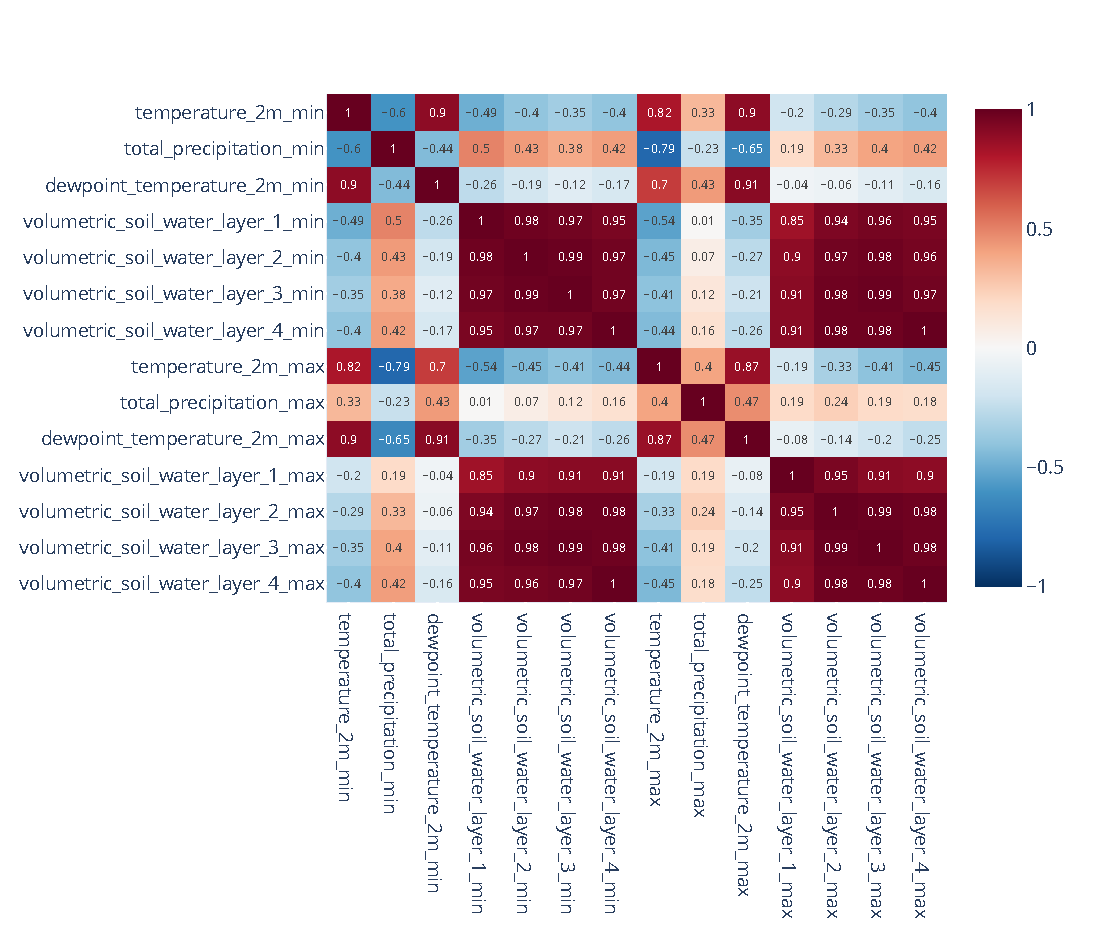
\includegraphics[width=0.96\linewidth, trim={20pt 20pt 10pt 40pt}, clip]{figures/figures_climate/weather_correlations.pdf}
    \caption{Correlations heatmap between various ERA5 variables. The data was downloaded from \cite{era5_dataset}, where detailed information is available.}
    \label{fig:weather_correlations}
\end{figure}

\section{Dataset Exploration}

As the ERA5 dataset contains numerous meteorological variables, a selection was made based on domain knowledge, correlations (Fig.\,\ref{fig:weather_correlations}), and studies such as \cite{climate_choice}. Fig.\,\ref{fig:selected_variables_stats} summarizes this selection, showing the median and quantiles for the aggregated dataset across all study locations using a representative median of the variables for the years 2010 to 2017. 

Fig.\,\ref{fig:selected_variables_stats} illustrates the significant variability within Europe, with the top-left plot indicating a difference of approximately 50\,K between the 1.0 quantile of minimum and maximum temperature measurements. This suggests that, although limited to Europe, this study explored a significant climate gradient. 

\begin{figure}[ht]
    \centering
    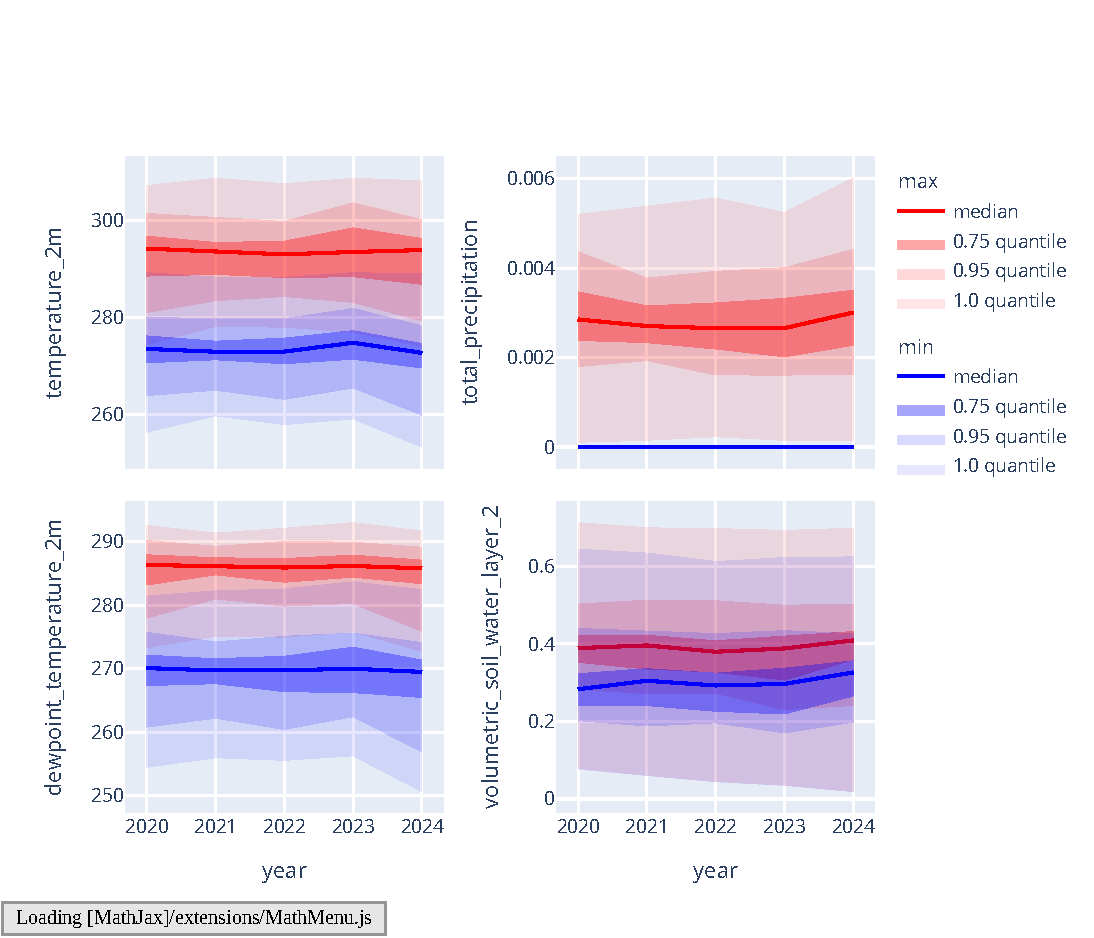
\includegraphics[width=0.98\linewidth, trim={20pt 20pt 10pt 40pt}, clip]{figures/figures_climate/selected_variables_stats.pdf}
    \caption{Median and quantiles of various monthly ERA5 variables by year.}
    \label{fig:selected_variables_stats}
\end{figure}
